%% Standalone lecture -- build with:  pdflatex -shell-escape ProbabilisticInference
%% Shared preamble for standalone lecture files.
%%
%% Every lecture begins with %% Shared preamble for standalone lecture files.
%%
%% Every lecture begins with %% Shared preamble for standalone lecture files.
%%
%% Every lecture begins with \input{preamble} and is compiled on its own:
%%     pdflatex -shell-escape <lecture>
%% There is no master lectures.tex any more -- the list of lectures lives in
%% lectures.yaml and is read by the build scripts.

\documentclass[25pt,landscape,footrule]{foils}
\input{macros_gen}
\backgroundsetup{contents={}}

\usepackage{stmaryrd}
\usepackage{ifthen}
\usepackage{pdf14}

% Every figure lives in this course's lectures/figures (consolidated
% 2026-10-08).  Do not add other courses' folders back: when a name exists in
% several folders LaTeX silently takes the first, which mixed old and new
% frames of the same animation.  A missing figure should be a build error.
\graphicspath{{figures/}{../lectures/figures/}}

\date{}

\newcounter{lessoncnt}
\newcommand{\lesson}[1]{\setcounter{page}{1}%
\section{Mathematics of Machine Learning\\%
\vfill
\textcolor{red}{\textit{#1}}
\vfill}}
 and is compiled on its own:
%%     pdflatex -shell-escape <lecture>
%% There is no master lectures.tex any more -- the list of lectures lives in
%% lectures.yaml and is read by the build scripts.

\documentclass[25pt,landscape,footrule]{foils}
%\usepackage[compat2,pdftex]{geometry}
\usepackage[pdftex]{geometry}
\geometry{headsep=-2.5ex,hscale=0.9,bmargin=2.5cm,tmargin=1cm,textwidth=25cm}
\usepackage[pdftex]{xcolor}
\usepackage{pause}
\usepackage{background}
%\usepackage[color=white]{background}
\usepackage{listings}
\usepackage{graphicx}
\usepackage{epsfig}
\usepackage{epstopdf}
\usepackage{bm}
\usepackage{amssymb}
\usepackage{amsfonts}
\usepackage{marvosym}
\usepackage{cite}
\usepackage{pifont}
\usepackage[english]{babel}
\usepackage{amsmath}
\usepackage{amsfonts}
\usepackage{rotating}
\usepackage{listings}
\usepackage{pp4slide}
%\usepackage{hyperref}
\usepackage{pp4link}
\usepackage{fancyvrb}
\usepackage{multido}
\usepackage{calc}
\usepackage{mleftright}
\mleftright % Redefines \left to \mleft and \right to \mright



\thinmuskip=1mu

\newcommand{\bigstrut}{\rule[-0.5\baselineskip]{0pt}{1.2\baselineskip}}
\renewcommand{\ttdefault}{pcr}

\newcommand{\squeeze}{\setlength{\itemsep}{-2pt}}
%\renewcommand{\familydefault}{cmr}
%\renewcommand{\labelitemii}{\textcolor{green}{$\star$}}
\newcommand{\tick}{{\large \ding{51}}}
\newcommand{\cross}{{\large \ding{55}}}
%\DeclareMathAlphabet{\mat}{OT1}{cmss}{bx}{n}
\DeclareMathAlphabet{\mat}{U}{eur}{b}{n}
\newcommand{\figs}{/home/apb/figures}
\newcommand{\stimes}{{\scriptstyle \times}}
\newcommand{\tr}{\textsf{T}}
\newcommand{\e}[1]{{\rm e}^{#1}}
\newcommand{\E}[1]{{\rm e}^{{\displaystyle #1}}}
\newcommand{\av}[2][]{\mathbb{E}_{#1}\left[ #2 \right]}
\newcommand{\Var}[1]{\mathbb{V}\mathrm{ar}\left( #1 \right)}
\newcommand{\pred}[1]{\left\llbracket { \small #1} \right\rrbracket}
\newcommand{\logg}[1]{\log\left( #1 \right)}
\newcommand{\logtwo}[1]{\log_2\left( #1 \right)}
\newcommand{\bra}[1]{\left( #1 \right)}
\newcommand{\prob}[1]{\mathbb{P}\left( #1 \right)}
\newcommand{\Prob}[1]{\mathbb{P}\left( #1 \right)}
\newcommand{\Step}{\mathop{\mat{\Theta}}}
\newcommand\diag{\mathop{\mathrm{diag}}}
\newcommand{\grad}{\bm{\nabla}}
\newcommand{\gradx}{\bm{\nabla}_{\!\!\scriptscriptstyle \bm{x}}}
\newcommand{\gradw}{\bm{\nabla}_{\!\!\scriptscriptstyle \bm{w}}}
\newcommand{\dd}{\mathrm{d}}
\newcommand{\ii}{\mathrm{i}}
\newcommand{\data}{\mathcal{D}}
\newcommand{\class}{\mathcal{C}}
\newcommand{\hypo}{\mathcal{H}}
\newcommand{\indep}{\perp \!\!\!\! \perp}
\newcommand{\pd}[3][\,]{\frac{\partial^{#1}{#2}}{\partial\,{#3}}}
\newcommand{\normal}[1]{\mathcal{N}\!\left( #1 \right)}
\newcommand{\Dist}[2][Binom]{\mathrm{#1}\left( \strut {#2} \right)}
\newcommand{\brackets}[1]{\!\left( #1 \right)}
\newcommand{\KL}[2]{\mathop{\mathrm{KL}}\left(#1 \big\| #2\right)}
\newcommand{\argmax}{\mathop{\mathrm{argmax}}}
\newcommand{\argmin}{\mathop{\mathrm{argmin}}}
\newcommand{\margin}{\Delta}
\lstnewenvironment{matlab}[1][frame=TB]{\lstset{#1}}{}       
%\renewcommand{\emph}[1]{\textcolor{red}{\textbf{#1}}}
\newcommand{\myskip}[1]{}
\newcommand\mycom[2]{\genfrac{}{}{0pt}{}{#1}{#2}}
\newcommand{\jl}{\lstinline[basicstyle=\ttfamily\color{DarkGreen},%
 keywordstyle=\bfseries\ttfamily\color{DarkGreen}]}
\definecolor{EmphColor}{rgb}{0.0,0.0,1.0}
\renewcommand{\emph}[1]{{\color{EmphColor}\textbf{#1}}}
\newcommand{\len}[1]{\| #1 \|}
\newcommand{\inner}[2]{\left\langle {#1}, {#2}\right\rangle}
\newenvironment{psmallmatrix}{\left(\begin{smallmatrix}}{\end{smallmatrix}\right)}
  

\definecolor{DarkGreen}{rgb}{0,0.5,0}
\definecolor{DarkRed}{rgb}{0,0,0.5}
\definecolor{HighLight}{rgb}{1,0,0}     % yellow
\definecolor{TextColor}{rgb}{0.0,0.1,0.1}     % white
\definecolor{TwoColor}{rgb}{0.0,0.5,0.1}      % used for switching colors

\definecolor{HeadLineColor}{rgb}{1.0,0.0,0.0} % cyan
\definecolor{SpecialColor}{rgb}{0.53,0.81,1.0}
\renewcommand{\normalcolor}{\color{HeadLineColor}}

\pausecolors{TwoColor}{TextColor}{HighLight}
\pausecolors{EmphColor}{TextColor}{EmphColor}
\pausecolors{DarkGreen}{DarkGreen}{DarkRed}
\pausecolors{SpecialColor}{white}{HighLight}

\newenvironment{PauseHighLight}{\color{TwoColor}\pausehighlight}{}
\newcommand{\multipdf}[2][width=\linewidth]{\multiinclude[pause=\pauselevel{:+0}\pause,format=pdf,graphics={#1}]{#2}}

\lstdefinelanguage{pseudo}
 {keywords={all,and,begin,break,continue,do,else,elseif,%
     end,endif,endfor,endwhile,%
     exit,false,for,forall,goto,if,%
     or,return,then,true,to,repeat,until,while},%
  comment=[s]{/*}{*/},%
  morecomment=[l]//,%
  morestring=[d]"%
 }[keywords,comments,strings]


\lstloadlanguages{Java,pseudo,Python}
\lstset{
  basicstyle=\footnotesize\ttfamily\color{DarkGreen},
  keywordstyle=\bfseries\footnotesize\ttfamily\color{DarkGreen},
  commentstyle=\footnotesize\it\rmfamily\color{blue},
  language=Java,
  showstringspaces=false
  }


\lstnewenvironment{pseudo}[1][]{\lstset{language=pseudo,mathescape,literate={:=}{{$\gets$}}2 {!}{{$\neg$}}1 {!=}{{\!\!$\neq$\,\,}}2 {<=}{{\!\!$\leq$\,\,}}2 {>=}{{\!\!$\geq$\,\,}}2,escapechar=\#,#1}}{}
\lstnewenvironment{java}[1][]{\lstset{escapechar=\$,#1}}{}
% Python code: the language setting makes # comments use commentstyle.
% Comments stay monospaced: the default italic roman letter-spaces badly
% on listings' fixed columns.
\lstnewenvironment{python}[1][frame=TB]{\lstset{language=Python,
    commentstyle=\footnotesize\ttfamily\color{blue},#1}}{}

\MyLogo{}
%\Restriction{}
%\rightfooter{\hyperlink{overview}{$\square$}}

\newcommand{\keywords}[1]{\vfill{\noindent\it #1}}

\newcounter{outlineitem}
\setcounter{outlineitem}{0}
\newcommand{\outlineitem}[2]{\item%
  \def\targ{\value{emumi}}%
  \ifnum\value{enumi}=\value{outlineitem}%
  \color{HighLight}\textbf{#1}\toptarget{#2}\color{TextColor}%
   \else\toplink{#2}{#1}\fi
}
\color{TwoColor}


%-- Instead of writing \section we want the file structured by \section.
\newcommand{\section}[2][0]{\foilhead[#1cm]{#2}}

%-- Write each page into a \begin{slide} -- \end{slide} environment.
\newenvironment{slide}{}{\pauselevel{=1}}

\MyLogo{\pauselevel{=1}\Acrobatmenu{GoBack}{%
  \color{TextColor}{Adam Pr\"ugel-Bennett}} \hspace{2cm}
  % Clicking on the name steps one slide back.
  \toplink{firstoutline}{\color{red}Mathematics of Machine
    Learning}%
  \hspace{2cm}
  \texttt{//ecs-vlc.github.io/aice3001/}
  %Clicking on the date jumps to the last page, which should be the
  %table of contents.
  \rightfooter{\Acrobatmenu{LastPage}{\qquad%
  \textsf{\color{TextColor}\tiny\thepage}}}% page number
  % Clicking on the page number steps one slide back.
}
\raggedright
\newcommand{\Outline}{}

\newcommand{\pb}{\pausebuild \color{TwoColor}}
\newcommand{\pauseb}{\pauselevel{build, highlight}\pause}
\newcommand{\hl}[1]{\pauselevel{=1, highlight =1 :1, highlight =#1 :#1}\pause}
\newcommand{\hll}{\pauselevel{=1, highlight =1 :1}\pause}
\newcommand{\pauseh}{\pauselevel{highlight}\pause}
\newcommand{\nhl}[1]{\textcolor{TextColor}{#1}}
\newcommand{\mypl}[1]{\pauselevel{=#1 :#1}\pause}
\input supp-pdf.tex
\DeclareGraphicsRule{*}{mps}{*}{}
\usepackage{mpmulti}
%\leftheader{}
\rightheader{} % no more page numbers on top right


\hypersetup{pdftitle={ECS Lectures},pdfsubject={Machine Learning}
pdfauthor={Adam Prugel-Bennett},pdfkeywords={machine learning},
pdfpagemode={FullScreen},
bookmarksopen=false,
hypertexnames=false,pdfstartview={FitV},colorlinks,linkcolor={blue},
citecolor={green},urlcolor={blue}}



\newcommand\bluepage{
\clearpage
\renewcommand\normalcolor{\color{yellow}}
\pagecolor{blue}
\renewcommand\Black{\color{white}}
\color{white}
\hypersetup{colorlinks=true}
}

\newcommand\whitepage{
\clearpage
\renewcommand\normalcolor{\color{black}}
\pagecolor{white}
\renewcommand\Black{\color{black}}
\color{black}
\hypersetup{colorlinks=true}
}

\whitepage
\setlength{\unitlength}{1mm}

\newenvironment{leftImage}[2][0.3]{%
\begin{minipage}{#1\linewidth}
  \includegraphics[width=\linewidth]{#2}
\end{minipage}\hfill
\begin{minipage}{0.92\linewidth - #1\linewidth}}%
{\end{minipage}}

\newenvironment{rightImage}[2][0.3]{%
\newcommand{\foot}{\begin{minipage}{#1\linewidth}\includegraphics[width=0.98\linewidth]{#2}\end{minipage}}%
\begin{minipage}{0.95\linewidth - #1\linewidth}\raggedright }{\end{minipage}\hfill\foot}


%%% Local Variables: 
%%% mode: latex
%%% TeX-master: t
%%% End: 

\backgroundsetup{contents={}}

\usepackage{stmaryrd}
\usepackage{ifthen}
\usepackage{pdf14}

% Every figure lives in this course's lectures/figures (consolidated
% 2026-10-08).  Do not add other courses' folders back: when a name exists in
% several folders LaTeX silently takes the first, which mixed old and new
% frames of the same animation.  A missing figure should be a build error.
\graphicspath{{figures/}{../lectures/figures/}}

\date{}

\newcounter{lessoncnt}
\newcommand{\lesson}[1]{\setcounter{page}{1}%
\section{Mathematics of Machine Learning\\%
\vfill
\textcolor{red}{\textit{#1}}
\vfill}}
 and is compiled on its own:
%%     pdflatex -shell-escape <lecture>
%% There is no master lectures.tex any more -- the list of lectures lives in
%% lectures.yaml and is read by the build scripts.

\documentclass[25pt,landscape,footrule]{foils}
%\usepackage[compat2,pdftex]{geometry}
\usepackage[pdftex]{geometry}
\geometry{headsep=-2.5ex,hscale=0.9,bmargin=2.5cm,tmargin=1cm,textwidth=25cm}
\usepackage[pdftex]{xcolor}
\usepackage{pause}
\usepackage{background}
%\usepackage[color=white]{background}
\usepackage{listings}
\usepackage{graphicx}
\usepackage{epsfig}
\usepackage{epstopdf}
\usepackage{bm}
\usepackage{amssymb}
\usepackage{amsfonts}
\usepackage{marvosym}
\usepackage{cite}
\usepackage{pifont}
\usepackage[english]{babel}
\usepackage{amsmath}
\usepackage{amsfonts}
\usepackage{rotating}
\usepackage{listings}
\usepackage{pp4slide}
%\usepackage{hyperref}
\usepackage{pp4link}
\usepackage{fancyvrb}
\usepackage{multido}
\usepackage{calc}
\usepackage{mleftright}
\mleftright % Redefines \left to \mleft and \right to \mright



\thinmuskip=1mu

\newcommand{\bigstrut}{\rule[-0.5\baselineskip]{0pt}{1.2\baselineskip}}
\renewcommand{\ttdefault}{pcr}

\newcommand{\squeeze}{\setlength{\itemsep}{-2pt}}
%\renewcommand{\familydefault}{cmr}
%\renewcommand{\labelitemii}{\textcolor{green}{$\star$}}
\newcommand{\tick}{{\large \ding{51}}}
\newcommand{\cross}{{\large \ding{55}}}
%\DeclareMathAlphabet{\mat}{OT1}{cmss}{bx}{n}
\DeclareMathAlphabet{\mat}{U}{eur}{b}{n}
\newcommand{\figs}{/home/apb/figures}
\newcommand{\stimes}{{\scriptstyle \times}}
\newcommand{\tr}{\textsf{T}}
\newcommand{\e}[1]{{\rm e}^{#1}}
\newcommand{\E}[1]{{\rm e}^{{\displaystyle #1}}}
\newcommand{\av}[2][]{\mathbb{E}_{#1}\left[ #2 \right]}
\newcommand{\Var}[1]{\mathbb{V}\mathrm{ar}\left( #1 \right)}
\newcommand{\pred}[1]{\left\llbracket { \small #1} \right\rrbracket}
\newcommand{\logg}[1]{\log\left( #1 \right)}
\newcommand{\logtwo}[1]{\log_2\left( #1 \right)}
\newcommand{\bra}[1]{\left( #1 \right)}
\newcommand{\prob}[1]{\mathbb{P}\left( #1 \right)}
\newcommand{\Prob}[1]{\mathbb{P}\left( #1 \right)}
\newcommand{\Step}{\mathop{\mat{\Theta}}}
\newcommand\diag{\mathop{\mathrm{diag}}}
\newcommand{\grad}{\bm{\nabla}}
\newcommand{\gradx}{\bm{\nabla}_{\!\!\scriptscriptstyle \bm{x}}}
\newcommand{\gradw}{\bm{\nabla}_{\!\!\scriptscriptstyle \bm{w}}}
\newcommand{\dd}{\mathrm{d}}
\newcommand{\ii}{\mathrm{i}}
\newcommand{\data}{\mathcal{D}}
\newcommand{\class}{\mathcal{C}}
\newcommand{\hypo}{\mathcal{H}}
\newcommand{\indep}{\perp \!\!\!\! \perp}
\newcommand{\pd}[3][\,]{\frac{\partial^{#1}{#2}}{\partial\,{#3}}}
\newcommand{\normal}[1]{\mathcal{N}\!\left( #1 \right)}
\newcommand{\Dist}[2][Binom]{\mathrm{#1}\left( \strut {#2} \right)}
\newcommand{\brackets}[1]{\!\left( #1 \right)}
\newcommand{\KL}[2]{\mathop{\mathrm{KL}}\left(#1 \big\| #2\right)}
\newcommand{\argmax}{\mathop{\mathrm{argmax}}}
\newcommand{\argmin}{\mathop{\mathrm{argmin}}}
\newcommand{\margin}{\Delta}
\lstnewenvironment{matlab}[1][frame=TB]{\lstset{#1}}{}       
%\renewcommand{\emph}[1]{\textcolor{red}{\textbf{#1}}}
\newcommand{\myskip}[1]{}
\newcommand\mycom[2]{\genfrac{}{}{0pt}{}{#1}{#2}}
\newcommand{\jl}{\lstinline[basicstyle=\ttfamily\color{DarkGreen},%
 keywordstyle=\bfseries\ttfamily\color{DarkGreen}]}
\definecolor{EmphColor}{rgb}{0.0,0.0,1.0}
\renewcommand{\emph}[1]{{\color{EmphColor}\textbf{#1}}}
\newcommand{\len}[1]{\| #1 \|}
\newcommand{\inner}[2]{\left\langle {#1}, {#2}\right\rangle}
\newenvironment{psmallmatrix}{\left(\begin{smallmatrix}}{\end{smallmatrix}\right)}
  

\definecolor{DarkGreen}{rgb}{0,0.5,0}
\definecolor{DarkRed}{rgb}{0,0,0.5}
\definecolor{HighLight}{rgb}{1,0,0}     % yellow
\definecolor{TextColor}{rgb}{0.0,0.1,0.1}     % white
\definecolor{TwoColor}{rgb}{0.0,0.5,0.1}      % used for switching colors

\definecolor{HeadLineColor}{rgb}{1.0,0.0,0.0} % cyan
\definecolor{SpecialColor}{rgb}{0.53,0.81,1.0}
\renewcommand{\normalcolor}{\color{HeadLineColor}}

\pausecolors{TwoColor}{TextColor}{HighLight}
\pausecolors{EmphColor}{TextColor}{EmphColor}
\pausecolors{DarkGreen}{DarkGreen}{DarkRed}
\pausecolors{SpecialColor}{white}{HighLight}

\newenvironment{PauseHighLight}{\color{TwoColor}\pausehighlight}{}
\newcommand{\multipdf}[2][width=\linewidth]{\multiinclude[pause=\pauselevel{:+0}\pause,format=pdf,graphics={#1}]{#2}}

\lstdefinelanguage{pseudo}
 {keywords={all,and,begin,break,continue,do,else,elseif,%
     end,endif,endfor,endwhile,%
     exit,false,for,forall,goto,if,%
     or,return,then,true,to,repeat,until,while},%
  comment=[s]{/*}{*/},%
  morecomment=[l]//,%
  morestring=[d]"%
 }[keywords,comments,strings]


\lstloadlanguages{Java,pseudo,Python}
\lstset{
  basicstyle=\footnotesize\ttfamily\color{DarkGreen},
  keywordstyle=\bfseries\footnotesize\ttfamily\color{DarkGreen},
  commentstyle=\footnotesize\it\rmfamily\color{blue},
  language=Java,
  showstringspaces=false
  }


\lstnewenvironment{pseudo}[1][]{\lstset{language=pseudo,mathescape,literate={:=}{{$\gets$}}2 {!}{{$\neg$}}1 {!=}{{\!\!$\neq$\,\,}}2 {<=}{{\!\!$\leq$\,\,}}2 {>=}{{\!\!$\geq$\,\,}}2,escapechar=\#,#1}}{}
\lstnewenvironment{java}[1][]{\lstset{escapechar=\$,#1}}{}
% Python code: the language setting makes # comments use commentstyle.
% Comments stay monospaced: the default italic roman letter-spaces badly
% on listings' fixed columns.
\lstnewenvironment{python}[1][frame=TB]{\lstset{language=Python,
    commentstyle=\footnotesize\ttfamily\color{blue},#1}}{}

\MyLogo{}
%\Restriction{}
%\rightfooter{\hyperlink{overview}{$\square$}}

\newcommand{\keywords}[1]{\vfill{\noindent\it #1}}

\newcounter{outlineitem}
\setcounter{outlineitem}{0}
\newcommand{\outlineitem}[2]{\item%
  \def\targ{\value{emumi}}%
  \ifnum\value{enumi}=\value{outlineitem}%
  \color{HighLight}\textbf{#1}\toptarget{#2}\color{TextColor}%
   \else\toplink{#2}{#1}\fi
}
\color{TwoColor}


%-- Instead of writing \section we want the file structured by \section.
\newcommand{\section}[2][0]{\foilhead[#1cm]{#2}}

%-- Write each page into a \begin{slide} -- \end{slide} environment.
\newenvironment{slide}{}{\pauselevel{=1}}

\MyLogo{\pauselevel{=1}\Acrobatmenu{GoBack}{%
  \color{TextColor}{Adam Pr\"ugel-Bennett}} \hspace{2cm}
  % Clicking on the name steps one slide back.
  \toplink{firstoutline}{\color{red}Mathematics of Machine
    Learning}%
  \hspace{2cm}
  \texttt{//ecs-vlc.github.io/aice3001/}
  %Clicking on the date jumps to the last page, which should be the
  %table of contents.
  \rightfooter{\Acrobatmenu{LastPage}{\qquad%
  \textsf{\color{TextColor}\tiny\thepage}}}% page number
  % Clicking on the page number steps one slide back.
}
\raggedright
\newcommand{\Outline}{}

\newcommand{\pb}{\pausebuild \color{TwoColor}}
\newcommand{\pauseb}{\pauselevel{build, highlight}\pause}
\newcommand{\hl}[1]{\pauselevel{=1, highlight =1 :1, highlight =#1 :#1}\pause}
\newcommand{\hll}{\pauselevel{=1, highlight =1 :1}\pause}
\newcommand{\pauseh}{\pauselevel{highlight}\pause}
\newcommand{\nhl}[1]{\textcolor{TextColor}{#1}}
\newcommand{\mypl}[1]{\pauselevel{=#1 :#1}\pause}
\input supp-pdf.tex
\DeclareGraphicsRule{*}{mps}{*}{}
\usepackage{mpmulti}
%\leftheader{}
\rightheader{} % no more page numbers on top right


\hypersetup{pdftitle={ECS Lectures},pdfsubject={Machine Learning}
pdfauthor={Adam Prugel-Bennett},pdfkeywords={machine learning},
pdfpagemode={FullScreen},
bookmarksopen=false,
hypertexnames=false,pdfstartview={FitV},colorlinks,linkcolor={blue},
citecolor={green},urlcolor={blue}}



\newcommand\bluepage{
\clearpage
\renewcommand\normalcolor{\color{yellow}}
\pagecolor{blue}
\renewcommand\Black{\color{white}}
\color{white}
\hypersetup{colorlinks=true}
}

\newcommand\whitepage{
\clearpage
\renewcommand\normalcolor{\color{black}}
\pagecolor{white}
\renewcommand\Black{\color{black}}
\color{black}
\hypersetup{colorlinks=true}
}

\whitepage
\setlength{\unitlength}{1mm}

\newenvironment{leftImage}[2][0.3]{%
\begin{minipage}{#1\linewidth}
  \includegraphics[width=\linewidth]{#2}
\end{minipage}\hfill
\begin{minipage}{0.92\linewidth - #1\linewidth}}%
{\end{minipage}}

\newenvironment{rightImage}[2][0.3]{%
\newcommand{\foot}{\begin{minipage}{#1\linewidth}\includegraphics[width=0.98\linewidth]{#2}\end{minipage}}%
\begin{minipage}{0.95\linewidth - #1\linewidth}\raggedright }{\end{minipage}\hfill\foot}


%%% Local Variables: 
%%% mode: latex
%%% TeX-master: t
%%% End: 

\backgroundsetup{contents={}}

\usepackage{stmaryrd}
\usepackage{ifthen}
\usepackage{pdf14}

% Every figure lives in this course's lectures/figures (consolidated
% 2026-10-08).  Do not add other courses' folders back: when a name exists in
% several folders LaTeX silently takes the first, which mixed old and new
% frames of the same animation.  A missing figure should be a build error.
\graphicspath{{figures/}{../lectures/figures/}}

\date{}

\newcounter{lessoncnt}
\newcommand{\lesson}[1]{\setcounter{page}{1}%
\section{Mathematics of Machine Learning\\%
\vfill
\textcolor{red}{\textit{#1}}
\vfill}}


\begin{document}

\lesson{Probabilistic Inference}
\vspace{-1cm}
\begin{center}
  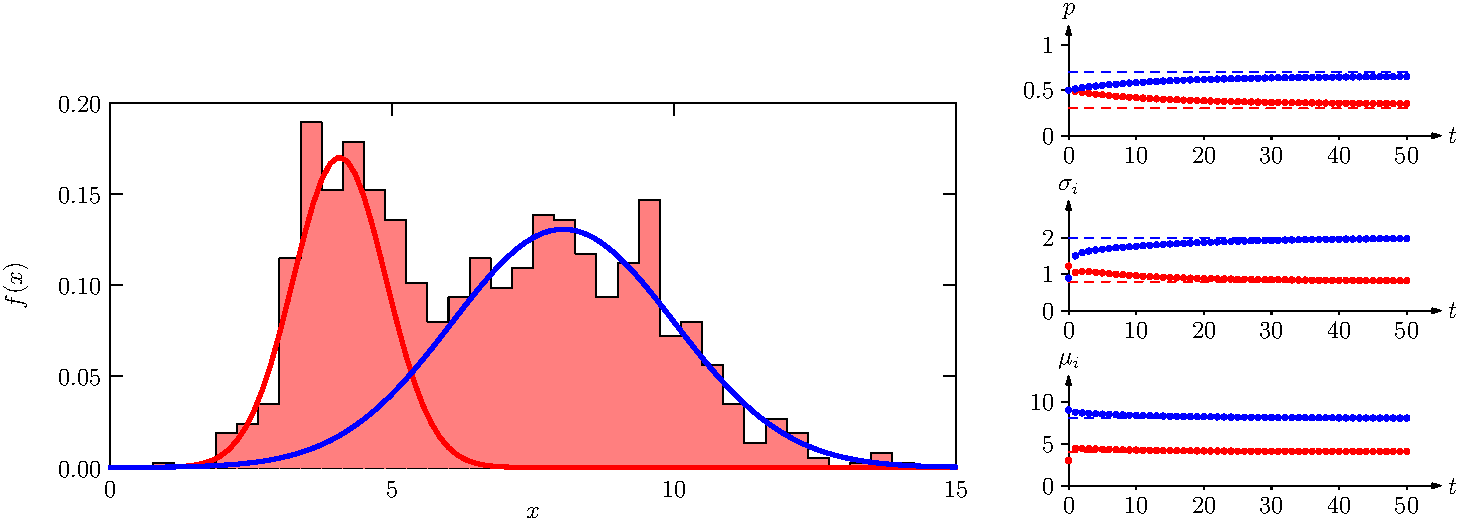
\includegraphics[width=\linewidth]{mog-1}
\end{center}
\keywords{Generative Models, Hierarchical Models, MAP, Empirical Bayes, Mixture of Gaussians, Expectation Maximisation}
%%%%%%%%%%%%%%%%%%%%%%% Next Slide %%%%%%%%%%%%%%%%%%%%%%%
\renewcommand{\Outline}{%
\begin{slide}
\section[1]{Outline}

\begin{minipage}{10cm}\raggedright
  \begin{enumerate}\squeeze
    \outlineitem{Building Probabilistic Models}{probmodel}
    \outlineitem{Hierarchical Models}{hier}
    \outlineitem{Solution Strategies}{strategies}
    \outlineitem{Mixtures and EM}{em}
  \end{enumerate}
\end{minipage}\hfill
\begin{minipage}{12cm}
  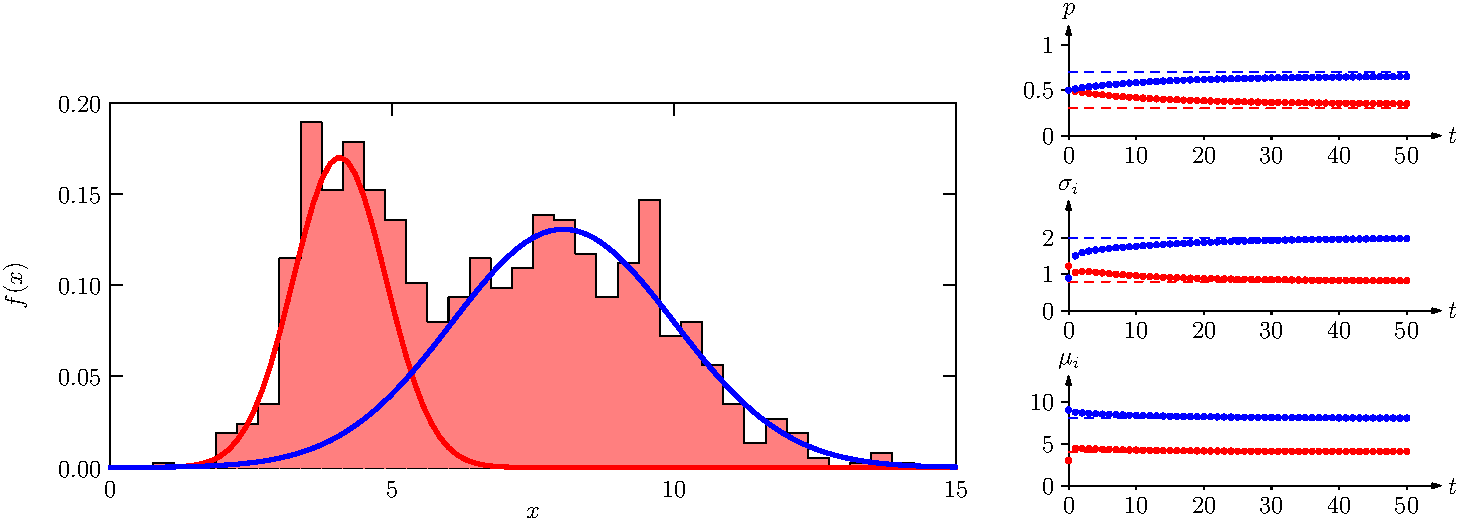
\includegraphics[width=12cm]{mog-1}
\end{minipage}
\end{slide}
\addtocounter{outlineitem}{1}
}

\setcounter{outlineitem}{1}
\Outline % Building Probabilistic Models
\toptarget{firstoutline}
%%%%%%%%%%%%%%%%%%%%%%% Next Slide %%%%%%%%%%%%%%%%%%%%%%%

\begin{slide}
\section{Beyond Conjugate Priors}

\begin{PauseHighLight}
  \begin{itemize}
  \item In the Bayes lecture we chose priors so that the posterior had
    the same form (conjugate priors)\pause
  \item Real problems have many interacting random variables, some of
    which we never observe, and the posterior has no closed form\pause
  \item This lecture: how to set up a probabilistic model, and simple
    strategies for using it (MAP, empirical Bayes, EM)\pause
  \item The MCMC lecture shows how to compute the full posterior\pause
  \end{itemize}
\end{PauseHighLight}

\end{slide}

%%%%%%%%%%%%%%%%%%%%%%% Next Slide %%%%%%%%%%%%%%%%%%%%%%%

\begin{slide}
\section{Two Rules}

\begin{PauseHighLight}
  \begin{itemize}
  \item Sum rule (marginalisation; see the probability lecture)
    \begin{align*}
      \Prob{X} = \sum_Y \Prob{X,Y} \qquad
      f(x) = \int f(x,y)\,\dd y\pause
    \end{align*}
  \item Product rule (the definition of conditional probability)
    \begin{align*}
      \Prob{X,Y} = \Prob{X|Y}\,\Prob{Y} = \Prob{Y|X}\,\Prob{X}\pause
    \end{align*}
  \item Bayes' rule is the product rule rearranged:
    $\Prob{X|Y} = \Prob{Y|X}\,\Prob{X}/\Prob{Y}$\pause
  \item Everything else follows from these two rules\pause
  \end{itemize}
\end{PauseHighLight}

\end{slide}

%%%%%%%%%%%%%%%%%%%%%%% Next Slide %%%%%%%%%%%%%%%%%%%%%%%

\begin{slide}
\section[-1]{Discriminative and Generative Models}

\begin{PauseHighLight}
  \begin{itemize}
  \item A \emph{discriminative model} gives the prediction directly,
    e.g.\ $\Prob{C|\bm{x}}$ for a class $C$ given features $\bm{x}$\pause{}
    (as for the Bayes' optimal discrimination surface in
    \textit{foundations of machine learning})\pauseb
  \item A \emph{generative model} describes how the features and the
    output are generated together: $\Prob{\bm{X},Y}$\pause
  \item Generative models are often more natural to think about\pause
  \item And we can still use them to discriminate
    \begin{align*}
      \Prob{Y|\bm{X}} = \frac{\Prob{\bm{X},Y}}{\Prob{\bm{X}}}
      = \frac{\Prob{\bm{X},Y}}{\sum\limits_Y \Prob{\bm{X}, Y}}\pause
    \end{align*}
  \end{itemize}
\end{PauseHighLight}

\end{slide}


%%%%%%%%%%%%%%%%%%%%%%% Next Slide %%%%%%%%%%%%%%%%%%%%%%%

\begin{slide}
\section{Latent Variables}

\begin{PauseHighLight}
  \begin{itemize}
  \item Sometimes we have models that involve random variables that we
    don't observe and we don't care about\pause
  \item These are called \emph{latent variables}\pause
  \item They are not observed and not our final target, but they make
    the model easy to write down\pause
  \item If we have a latent variable $Z$ and observed variable $\bm{X}$
    and we are predicting a variable $Y$ then we would
    \emph{marginalise} over the latent variable
    \begin{align*}
      \Prob{\bm{X}, Y} = \sum_Z \Prob{\bm{X}, Y, Z}\pause
    \end{align*}
  \end{itemize}
\end{PauseHighLight}

\end{slide}

%%%%%%%%%%%%%%%%%%%%%%% Next Slide %%%%%%%%%%%%%%%%%%%%%%%

\begin{slide}
\section[-2]{Generative Stories}

\begin{PauseHighLight}
  \begin{itemize}\squeeze
  \item Build a model by writing down how the data could have been
    generated (a simulator), each line drawing one variable given
    earlier ones\pause
\begin{python}
theta = rng.beta(a, b, size=J)    # a rate for each product
k = rng.binomial(n, theta)        # observed positive reviews
\end{python}\pause
  \item The joint distribution is the product of the lines (product
    rule)
    \begin{align*}
      f(\bm{\theta},\bm{k}) = \prod_{j=1}^J
      \mathrm{Beta}(\theta_j|a,b)\,\mathrm{Bin}(k_j|n_j,\theta_j)\pause
    \end{align*}
  \item \emph{Probabilistic programming languages} (e.g.\ Stan, PyMC)
    take such a programme and do the inference for you\pause
  \end{itemize}
\end{PauseHighLight}

\end{slide}

%%%%%%%%%%%%%%%%%%%%%%% Next Slide %%%%%%%%%%%%%%%%%%%%%%%
\Outline % Hierarchical Models
%%%%%%%%%%%%%%%%%%%%%%% Next Slide %%%%%%%%%%%%%%%%%%%%%%%

\begin{slide}
\section{Rating Products}

\begin{PauseHighLight}
  \begin{itemize}
  \item A shop lists products with the fraction of positive
    reviews: which is better?\pause
    \begin{center}
      \begin{tabular}{l|cc}
        & positive & fraction \\ \hline
        Product $A$ & 3 of 3 & 100\% \\
        Product $B$ & 1840 of 2000 & 92\%
      \end{tabular}
    \end{center}\pause
  \item Ranking by the fraction puts every product with a handful of
    good reviews at the top\pause
  \item Intuitively we should trust $A$'s 100\% less\pause{}, and
    something like ``most products are rated about 80\%'' should pull
    it down\pauseb{}: a hierarchical model makes this precise\pauseb
  \end{itemize}
\end{PauseHighLight}

\end{slide}

%%%%%%%%%%%%%%%%%%%%%%% Next Slide %%%%%%%%%%%%%%%%%%%%%%%

\begin{slide}
\section[-1]{A Model for Ratings}

\begin{PauseHighLight}
  \begin{itemize}
  \item Product $j$ has an unknown probability $\theta_j$ that a review
    is positive; $k_j$ of its $n_j$ reviews are positive
    \begin{align*}
      k_j \sim \mathrm{Bin}(n_j, \theta_j)\pause
    \end{align*}
  \item The products are different but similar: their $\theta_j$ come
    from a common population
    \begin{align*}
      \theta_j \sim \mathrm{Beta}(a, b)\pause
    \end{align*}
  \item The \emph{hyperparameters} $a$, $b$ describe the population:
    $a/(a+b)$ is the typical rate and $a+b$ measures how alike the
    products are\pause
  \item The model has levels: population $\rightarrow$ product
    $\rightarrow$ reviews\pause{} (a \emph{hierarchical model})\pauseb
  \end{itemize}
\end{PauseHighLight}

\end{slide}

%%%%%%%%%%%%%%%%%%%%%%% Next Slide %%%%%%%%%%%%%%%%%%%%%%%

\begin{slide}
\section[-1]{Graphical Models}

\begin{PauseHighLight}
  \begin{center}
    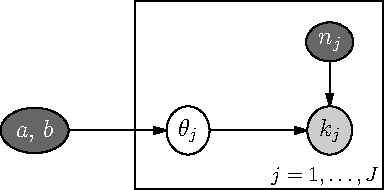
\includegraphics[width=0.5\linewidth]{gmModels-0}\pause
  \end{center}
  \begin{itemize}\squeeze
  \item Nodes are variables (dark: fixed; shaded: observed; white:
    latent); arrows point from the variables each one is drawn from\pause
  \item A box (a \emph{plate}) means ``repeat for each $j$''\pause
  \item The joint distribution is the product over nodes of each
    node given its parents\pause
  \item Diagrams like this are a good way to design and explain models\pause
  \end{itemize}
\end{PauseHighLight}

\end{slide}

%%%%%%%%%%%%%%%%%%%%%%% Next Slide %%%%%%%%%%%%%%%%%%%%%%%

\begin{slide}
\section[-1]{One Product at a Time}

\begin{PauseHighLight}
  \begin{itemize}
  \item If we knew $a$ and $b$, each product is a beta-binomial problem
    from the Bayes lecture
    \begin{align*}
      f(\theta_j|k_j) = \mathrm{Beta}(\theta_j|a+k_j, b+n_j-k_j)\pause
    \end{align*}
  \item The posterior mean is a weighted average: the prior counts as
    $a+b$ extra reviews
    \begin{align*}
      \av{\theta_j|k_j} = \frac{a+k_j}{a+b+n_j}
      = \frac{a+b}{a+b+n_j}\,\frac{a}{a+b} +
      \frac{n_j}{a+b+n_j}\,\frac{k_j}{n_j}\pause
    \end{align*}
  \item With $a=20$, $b=5$ (typical rate 0.8, worth 25 reviews):
    $A$ gets $23/28 = 0.82$\pause{} and $B$ gets $1860/2025 =
    0.92$\pauseb{}: $B$ is better\pauseb
  \end{itemize}
\end{PauseHighLight}

\end{slide}

%%%%%%%%%%%%%%%%%%%%%%% Next Slide %%%%%%%%%%%%%%%%%%%%%%%

\begin{slide}
\section[-2]{Shrinkage}

\pb\pause\pauselevel{=1}
\begin{center}
  \multipdf[width=0.8\linewidth]{ratingsShrink}\pause
\end{center}
Few reviews: pulled (\emph{shrunk}) to the typical rate; many: barely
move.  Products \emph{borrow strength} from each other.\pauseh

\end{slide}

%%%%%%%%%%%%%%%%%%%%%%% Next Slide %%%%%%%%%%%%%%%%%%%%%%%

\begin{slide}
\section{Partial Pooling}

\begin{PauseHighLight}
  \begin{itemize}
  \item Two extremes
    \begin{itemize}
    \item no pooling: estimate each product alone ($k_j/n_j$)\pause{}
      ---noisy when $n_j$ is small\pauseb
    \item complete pooling: assume all products are the same\pause{}
      ---ignores real differences\pauseb
    \end{itemize}
  \item The hierarchical model sits in between, and the data decide
    where (through $a+b$)\pause
  \item The same idea appears everywhere: schools, hospitals, adverts,
    players, users of a recommender\pause
  \item But we don't know $a$ and $b$, and with them unknown the
    posterior $f(a,b,\bm{\theta}|\bm{k})$ has no closed form\pause
  \end{itemize}
\end{PauseHighLight}

\end{slide}

%%%%%%%%%%%%%%%%%%%%%%% Next Slide %%%%%%%%%%%%%%%%%%%%%%%
\Outline % Solution Strategies
%%%%%%%%%%%%%%%%%%%%%%% Next Slide %%%%%%%%%%%%%%%%%%%%%%%

\begin{slide}
\section[-1]{Full Bayesian Inference}

\begin{PauseHighLight}
  \begin{itemize}
  \item Bayes' rule gives the posterior over the parameters
    \begin{align*}
      \Prob{\bm{\Theta}|\mathcal{D}} =
      \frac{\Prob{\mathcal{D}|\bm{\Theta}}\, \Prob{\bm{\Theta}}}{
      \Prob{\mathcal{D}} }\pause
    \end{align*}
  \item It describes its own uncertainty and is much less prone to
    over-fitting (we average over parameters rather than choosing the
    best)\pause
  \item But the posterior is rarely a nice function, and its
    normalisation, the \textit{evidence}
    $\Prob{\mathcal{D}} = \sum_{\bm{\Theta}}
    \Prob{\mathcal{D}|\bm{\Theta}}\, \Prob{\bm{\Theta}}$, is a sum over
    far too many values\pause
  \item Monte Carlo methods (the MCMC lecture) can sample from the
    posterior without computing $\Prob{\mathcal{D}}$\pause
  \end{itemize}
\end{PauseHighLight}

\end{slide}

%%%%%%%%%%%%%%%%%%%%%%% Next Slide %%%%%%%%%%%%%%%%%%%%%%%

\begin{slide}
\section[-1]{Maximum A Posteriori (MAP) Solution}

\begin{PauseHighLight}
  \begin{itemize}
  \item Work around: the mode of the posterior (no need for $f(\mathcal{D})$)
    \begin{align*}
       \hspace{-1cm}\bm{\Theta}_{\text{\small MAP}} =
      \argmax_{\bm{\Theta}} \,
       f(\mathcal{D}|\bm{\Theta})\, f(\bm{\Theta})  =
       \argmax_{\bm{\Theta}} \, \logg{f(\mathcal{D}|\bm{\Theta})} +
       \logg{f(\bm{\Theta})}\pause
    \end{align*}
  \item $-\logg{f(\bm{\Theta})}$ acts as a regulariser: a Gaussian
    prior on weights gives $\|\bm{w}\|^2$, i.e.\ ridge regression or
    weight decay\pause{} (we use this in the next lecture)\pauseb
  \item With a uniform prior MAP is \emph{maximum likelihood}\pause{}:
    often sufficient for \textit{government work}\pauseb
  \item Neither is Bayesian\pause{} (despite what you are sometimes
    told)\pauseb: they can overfit and give no error estimate\pauseb
  \end{itemize}
\end{PauseHighLight}

\end{slide}

%%%%%%%%%%%%%%%%%%%%%%% Next Slide %%%%%%%%%%%%%%%%%%%%%%%

\begin{slide}
\section[-2]{Empirical Bayes}

\begin{PauseHighLight}
  \begin{itemize}\squeeze
  \item A half-way house: integrate out the many $\theta_j$, optimise
    the few hyperparameters, then use the conjugate posteriors\pause
  \item For the ratings model the integral is in closed form (the
    \emph{beta-binomial})
    \begin{align*}
      \Prob{k_j|a,b} &= \int_0^1 \mathrm{Bin}(k_j|n_j,\theta)\,
      \mathrm{Beta}(\theta|a,b)\,\dd\theta \\
      &= \binom{n_j}{k_j}\frac{B(a+k_j,\,b+n_j-k_j)}{B(a,b)}\pause
    \end{align*}
  \item Choose $a$, $b$ to maximise the evidence
    $\prod_j\Prob{k_j|a,b}$ (as for the GP hyperparameters)\pause{}:
    for the data in the figure $a=19.9$, $b=5.3$\pauseb
  \item Cheap and often good, but ignores uncertainty in $a$, $b$\pause
  \end{itemize}
\end{PauseHighLight}

\end{slide}

%%%%%%%%%%%%%%%%%%%%%%% Next Slide %%%%%%%%%%%%%%%%%%%%%%%

\begin{slide}
\section{A Ladder of Strategies}

\begin{PauseHighLight}
  \begin{center}
    \begin{tabular}{l|l|l}
      Strategy & What you get & Cost \\ \hline
      ML & a point estimate & optimiser\pause \\
      MAP & a regularised point & optimiser\pause \\
      Empirical Bayes & posteriors given $a,b$ & an integral\pause \\
      EM & ML/MAP with latents & iterate\pause \\
      Full Bayes & all the uncertainty & MCMC\pause
    \end{tabular}
  \end{center}
  \begin{itemize}
  \item Choose the cheapest that answers your question\pause
  \item The rest of this lecture: EM\pause
  \end{itemize}
\end{PauseHighLight}

\end{slide}

%%%%%%%%%%%%%%%%%%%%%%% Next Slide %%%%%%%%%%%%%%%%%%%%%%%
\Outline % Mixtures and EM
%%%%%%%%%%%%%%%%%%%%%%% Next Slide %%%%%%%%%%%%%%%%%%%%%%%

\begin{slide}
\section{You Already Know EM}

\begin{PauseHighLight}
  \begin{itemize}
  \item $k$-means clustering
    \begin{enumerate}
    \item assign each point to its nearest centre\pause
    \item move each centre to the mean of its points\pause
    \item repeat\pause
    \end{enumerate}
  \item Step 1 guesses the hidden cluster labels; step 2 fits the
    parameters as if those guesses were right\pause
  \item The EM algorithm does the same with \emph{probabilities} of
    belonging to each cluster\pause
  \item It comes from a probabilistic model: a mixture\pause
  \end{itemize}
\end{PauseHighLight}

\end{slide}

%%%%%%%%%%%%%%%%%%%%%%% Next Slide %%%%%%%%%%%%%%%%%%%%%%%

\begin{slide}
\section{Mixture of Gaussians}

\begin{PauseHighLight}
  \begin{itemize}
  \item Suppose we detect two types of short-lived particle, $A$ or
    $B$, and measure each particle's mass, $X_i$, with a noisy
    detector, but not its type\pause
  \item Let $Z_i\in\{0,1\}$ indicate that particle $i$ is of type $A$,
    with $\Prob{Z_i=1}=p$\pause
  \item $X_i$ is normal with unknown means and variances, so the
    parameters are $\bm{\Theta} = (\mu_A, \sigma_A^2, \mu_B, \sigma_B^2, p)$\pause
  \item The probability of $X_i$ is given by
    \begin{align*}
      f(X_i|Z_i,\bm{\Theta}) = Z_i\,\normal{X_i\big|\mu_A,\sigma_A^2} +
      (1-Z_i)\,\normal{X_i\big|\mu_B,\sigma_B^2}\pause
    \end{align*}
  \end{itemize}
\end{PauseHighLight}

\end{slide}

%%%%%%%%%%%%%%%%%%%%%%% Next Slide %%%%%%%%%%%%%%%%%%%%%%%

\begin{slide}
\section[-1]{Mixture as a Graphical Model}

\begin{PauseHighLight}
  \begin{center}
    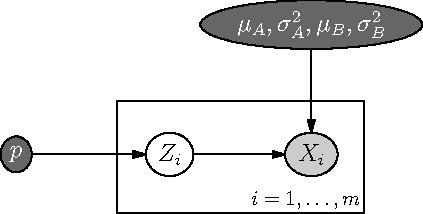
\includegraphics[width=0.55\linewidth]{gmModels-1}\pause
  \end{center}
  \begin{itemize}
  \item For each data point draw a type $Z_i$, then a mass $X_i$ from
    that type's normal distribution\pause
  \item $Z_i$ is latent: we must marginalise it out\pause
  \item The parameters (dark) are shared by all data points, so they
    sit outside the plate\pause
  \end{itemize}
\end{PauseHighLight}

\end{slide}

%%%%%%%%%%%%%%%%%%%%%%% Next Slide %%%%%%%%%%%%%%%%%%%%%%%

\begin{slide}
\section[-2]{Data}

\begin{PauseHighLight}
  \begin{itemize}
  \item Note that{\small
    \begin{align*}
      f(X_i|\bm{\Theta})
      &= \sum_{Z_i\in\{0,1\}} f(X_i,Z_i|\bm{\Theta})\pause
        = \sum_{Z_i\in\{0,1\}}
        f(X_i|Z_i,\bm{\Theta})\,\Prob{Z_i}\pause \\
      &= \av[Z_i]{f(X_i|Z_i,\bm{\Theta})}\pause
      = p \, \normal{X_i\big|\mu_A,\sigma_A^2} +
      (1-p)\,\normal{X_i\big|\mu_B,\sigma_B^2}\pause
    \end{align*}}
  \end{itemize}
  \begin{center}
    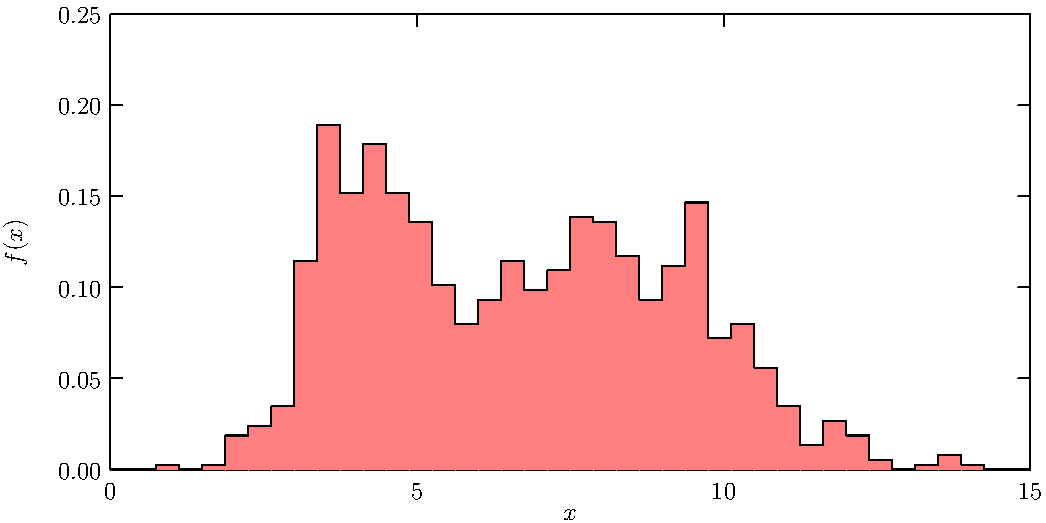
\includegraphics[width=0.8\linewidth]{mixtureOfGaussiansData}\pause
  \end{center}
\end{PauseHighLight}

\end{slide}

%%%%%%%%%%%%%%%%%%%%%%% Next Slide %%%%%%%%%%%%%%%%%%%%%%%

\begin{slide}
\section[-1]{Maximum Likelihood}

\begin{PauseHighLight}
  \begin{itemize}
  \item A full Bayesian treatment needs priors on $\bm{\Theta}$ and
    would give a distribution over parameters\pause
  \item Often we only want a reasonable estimate for some of our
    parameters (e.g. the masses $\mu_A$ and $\mu_B$)\pause
  \item A reasonable approach is to seek those parameters that maximise the
    likelihood of our observed data (assumed independent)
    \begin{align*}
      f(\data|\bm{\Theta}) = \prod_{X\in\data} f(X|\bm{\Theta})\pause
    \end{align*}
  \item {\small Strictly, we seek a good \emph{local} maximum: putting
      $\mu_A=X_1$ and letting $\sigma_A\to0$ makes the likelihood
      infinite}\pause
  \end{itemize}
\end{PauseHighLight}

\end{slide}

%%%%%%%%%%%%%%%%%%%%%%% Next Slide %%%%%%%%%%%%%%%%%%%%%%%

\begin{slide}
\section[-1]{EM Algorithm}

\begin{PauseHighLight}
  \begin{itemize}
  \item If we knew each particle's type, $Z_i$, maximising the
    likelihood would be easy\pause{}; but estimating $\Prob{Z_i=1|X_i}$
    needs the parameters\pauseb
  \item The \emph{expectation-maximisation} (EM) algorithm iterates:
    maximise the log-likelihood of the data \emph{and} latent
    variables, averaged over the latent variables using the current
    parameters
    \begin{align*}
      \bm{\Theta}^{(t+1)} = \mathop{\mathrm{argmax}}_{\bm{\Theta}}
      \sum_{\bm{Z}} \Prob{\bm{Z}\big|\data,\bm{\Theta}^{(t)}}\,
      \logg{f(\data,\bm{Z}| \bm{\Theta})}\pause
    \end{align*}
  \item E-step: compute $\Prob{\bm{Z}|\data,\bm{\Theta}^{(t)}}$;
    M-step: maximise\pause
  \item No step decreases the likelihood\pause{} (the proof is in the
    notes)\pauseb
  \end{itemize}
\end{PauseHighLight}

\end{slide}

%%%%%%%%%%%%%%%%%%%%%%% Next Slide %%%%%%%%%%%%%%%%%%%%%%%

\begin{slide}
\section[-1]{E-Step: Responsibilities}

\begin{PauseHighLight}
  \begin{itemize}
  \item We need the distribution of the latent variables
    conditioned on the data and current estimated parameters\pause
  \item For our problem
    \begin{align*}
      \Prob{\bm{Z}\big|\data,\bm{\Theta}^{(t)}} =
      \prod_{i=1}^m \Prob{Z_i\big|X_i,\bm{\Theta}^{(t)}}\pause
    \end{align*}
    where, by Bayes' rule, the \emph{responsibility} of type $A$ for
    point $i$ is {\small
    \begin{align*}
      \gamma_i^{(t)} = \Prob{Z_i=1\big|X_i,\bm{\Theta}^{(t)}} &= \frac{p^{(t)}\,
      \normal{X_i\big|\mu_A^{(t)},\sigma_A^{2(t)}} }
     { p^{(t)}\,\normal{X_i\big|\mu_A^{(t)},\sigma_A^{2(t)}} +
     (1-p^{(t)})\, \normal{X_i\big|\mu_B^{(t)},\sigma_B^{2(t)}} }
    \end{align*}}
    and $\Prob{Z_i=0\big|X_i,\bm{\Theta}^{(t)}} = 1 - \gamma_i^{(t)}$\pause
  \end{itemize}
\end{PauseHighLight}


\end{slide}

%%%%%%%%%%%%%%%%%%%%%%% Next Slide %%%%%%%%%%%%%%%%%%%%%%%

\begin{slide}
\section[-1]{M-Step}

\begin{PauseHighLight}
  \begin{itemize}
  \item The data points are independent, so
    {\small
      \begin{align*}
       Q(\bm{\Theta}|\bm{\Theta}^{(t)})
      &= \sum_{i=1}^m \Bigl[ \gamma_i^{(t)} \Bigl( \log(p) -
        \frac{(X_i-\mu_A)^2}{2\,\sigma^2_A} - \tfrac12\logg{2\,\pi\,\sigma^2_A}
        \Bigr) \\
      & \hspace{1.5cm} + (1-\gamma_i^{(t)}) \Bigl( \log(1-p) -
        \frac{(X_i-\mu_B)^2}{2\,\sigma^2_B} - \tfrac12\logg{2\,\pi\,\sigma^2_B}
        \Bigr)\Bigr]\pause
    \end{align*} }
  \item For example, only the first bracket involves $\mu_A$
    \begin{align*}
      \pd{Q}{\mu_A} = \sum_{i=1}^m \gamma_i^{(t)}\,
      \frac{X_i-\mu_A}{\sigma_A^2} = 0
      \quad\Rightarrow\quad
      \mu_A^{(t+1)} = \frac{ \sum_{i=1}^m \gamma_i^{(t)}\, X_i}
        {\sum_{i=1}^m \gamma_i^{(t)}}\pause
    \end{align*}
  \item The other parameters work the same way (see the notes)\pause
  \end{itemize}
\end{PauseHighLight}

\end{slide}

%%%%%%%%%%%%%%%%%%%%%%% Next Slide %%%%%%%%%%%%%%%%%%%%%%%

\begin{slide}
\section[-2]{Update Equations}

\begin{PauseHighLight}
  \begin{itemize}
  \item Fraction of type $A$: the average responsibility
    \begin{align*}
      p^{(t+1)} = \frac{1}{m} \sum_{i=1}^m \gamma_i^{(t)}\pause
    \end{align*}
  \item Means: weighted averages of the data
    \begin{align*}
      \mu_A^{(t+1)}
      &= \frac{ \sum_{i=1}^m \gamma_i^{(t)}\, X_i}
        {\sum_{i=1}^m \gamma_i^{(t)}}, &
      \mu_B^{(t+1)}
      &= \frac{ \sum_{i=1}^m (1-\gamma_i^{(t)})\, X_i}
        {\sum_{i=1}^m (1-\gamma_i^{(t)})}\pause
    \end{align*}
  \item Variances: weighted variances (if every $\gamma_i$ were 0 or 1,
    these would all be the ordinary group statistics)
  \begin{align*}
    \sigma_A^{2(t+1)}
      = \frac{ \sum_{i=1}^m \gamma_i^{(t)}
        (X_i-\mu^{(t+1)}_A)^2}
        {\sum_{i=1}^m \gamma_i^{(t)}}\pause
  \end{align*}
  \end{itemize}
\end{PauseHighLight}

\end{slide}

%%%%%%%%%%%%%%%%%%%%%%% Next Slide %%%%%%%%%%%%%%%%%%%%%%%

\begin{slide}
\section{Example}
\pause
\pb\pauselevel{=1}
\begin{center}
  \multipdf[width=\linewidth]{mixtureOfGaussians}\pause
\end{center}
\end{slide}

%%%%%%%%%%%%%%%%%%%%%%% Next Slide %%%%%%%%%%%%%%%%%%%%%%%

\begin{slide}
\section{EM in Practice}

\begin{PauseHighLight}
  \begin{itemize}
  \item With equal, fixed variances and $\sigma\to0$ the
    responsibilities become 0 or 1: EM becomes $k$-means\pause
  \item EM finds a local maximum: run it from several starts\pause
  \item A component can collapse onto a single point ($\sigma\to0$,
    likelihood $\to\infty$)\pause{}: a prior on $\sigma$ (i.e.\ MAP)
    prevents this\pauseb
  \item Convergence can be slow when the components overlap (the
    latent variables are very uncertain)\pause
  \item Simple updates, no step size, and it works for any model with
    latent variables (missing data, hidden Markov models, \ldots)\pause
  \end{itemize}
\end{PauseHighLight}

\end{slide}

%%%%%%%%%%%%%%%%%%%%%%% Next Slide %%%%%%%%%%%%%%%%%%%%%%%

\begin{slide}
\section{Summary}

\begin{PauseHighLight}
  \begin{itemize}
  \item Build a model by writing down how the data were generated: a
    generative story or graphical model\pause
  \item Hierarchical models let similar groups share strength
    (shrinkage)\pause
  \item Beyond conjugate priors there is a ladder of strategies:
    ML, MAP, empirical Bayes, EM, full Bayes with MCMC\pause
  \item The EM algorithm maximises likelihoods (or MAP) when there are
    latent variables\pause
  \item It gives nice update equations, but finds local optima and can
    converge slowly\pause
  \end{itemize}
\end{PauseHighLight}

\end{slide}


%%% Local Variables:
%%% TeX-master: "lectures"
%%% End:

\end{document}
